%\usetikzlibrary{backgrounds} % DEBUG
%background rectangle/.style={fill=olive!45}, show background rectangle
\begin{figure}
	\centering
	\begin{minipage}[t]{1.0\textwidth}
		\hspace{20pt}
		\begin{tikzpicture}[scale=1, trim axis left, trim axis right]
			\begin{axis}[xlabel=$t$, ylabel=$\langle\hat{\sigma}_z\rangle$, grid=both, grid style={gray!20}, every axis plot/.append style={very thick}, scale only axis, height=\globalQuenchLargeFieldFigureHeight, width=\globalQuenchLargeFieldFigureWidth, xmin=-0.05, xmax=1.05, ymin=-1.1, ymax=1.1, legend style={nodes={scale=\legendscale, transform shape, font=\small}}, legend pos=south east]
				%	
				\addplot[color = 5blue1]
				table[x=t_tenpy, y=sz_chi_16, col sep=space]{figures/plots/TFI/global_quench/data/global_quench_g_6.0_tenpy_site_index_4_4_0.txt};
				\addlegendentry{$\chi= 16$}
				%	
				\addplot[color = 5blue2]
				table[x=t_tenpy, y=sz_chi_32, col sep=space]{figures/plots/TFI/global_quench/data/global_quench_g_6.0_tenpy_site_index_4_4_0.txt};
				\addlegendentry{$\chi= 32$}
				%	
				\addplot[color = 5blue3]
				table[x=t_tenpy, y=sz_chi_64, col sep=space]{figures/plots/TFI/global_quench/data/global_quench_g_6.0_tenpy_site_index_4_4_0.txt};
				\addlegendentry{$\chi= 64$}
				%	
				\addplot[color = 5blue4]
				table[x=t_tenpy, y=sz_chi_128, col sep=space]{figures/plots/TFI/global_quench/data/global_quench_g_6.0_tenpy_site_index_4_4_0.txt};
				\addlegendentry{$\chi= 128$}
				%	
				\addplot[color = 5blue5]
				table[x=t_tenpy, y=sz_chi_256, col sep=space]{figures/plots/TFI/global_quench/data/global_quench_g_6.0_tenpy_site_index_4_4_0.txt};
				\addlegendentry{$\chi= 256$}
				%
			\end{axis}%
			\begin{axis}[scale only axis, height=\globalQuenchLargeFieldFigureHeight, width=\globalQuenchLargeFieldFigureWidth, every axis plot/.append style={very thick}, xmin=-0.05, xmax=1.05, ymin=-1.1, ymax=1.1, legend style={nodes={scale=\legendscale, transform shape, font=\small}}, legend pos=north west]
				%	
				\addplot[color = 3red1]
				table[x=t_disoTPS, y=sz_disoTPS_D_2, col sep=space]{figures/plots/TFI/global_quench/data/global_quench_g_6.0_disoTPS_site_index_4_4_0.txt};
				\addlegendentry{$D = 2$}
				%	
				\addplot[color = 3red2]
				table[x=t_disoTPS, y=sz_disoTPS_D_4, col sep=space]{figures/plots/TFI/global_quench/data/global_quench_g_6.0_disoTPS_site_index_4_4_0.txt};
				\addlegendentry{$D = 4$}
				%	
				\addplot[color = 3red3]
				table[x=t_disoTPS, y=sz_disoTPS_D_6, col sep=space]{figures/plots/TFI/global_quench/data/global_quench_g_6.0_disoTPS_site_index_4_4_0.txt};
				\addlegendentry{$D = 6$}
				%
			\end{axis}%
		\end{tikzpicture}%
		\quad
		\raisebox{34.2pt}
		{%
			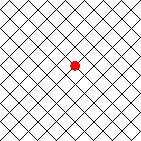
\includegraphics[scale=1.1]{figures/tikz/TFI/site_indices/site_index_a.pdf}
		}
	\end{minipage}	
	\par\medskip
	\begin{minipage}{1.0\textwidth}
		\hspace{20pt}
		\begin{tikzpicture}[scale=1, trim axis left, trim axis right]
			\begin{axis}[xlabel=$t$, ylabel=$\langle\hat{\sigma}_z\rangle$, grid=both, grid style={gray!20}, every axis plot/.append style={very thick}, scale only axis, height=\globalQuenchLargeFieldFigureHeight, width=\globalQuenchLargeFieldFigureWidth, xmin=-0.05, xmax=1.05, ymin=0.5, ymax=1.1]
				%	
				\addplot[color = 5blue1]
				table[x=t_tenpy, y=sz_chi_16, col sep=space]{figures/plots/TFI/global_quench/data/global_quench_g_6.0_tenpy_site_index_4_4_1.txt};
				%\addlegendentry{$\chi= 16$}
				%	
				\addplot[color = 5blue2]
				table[x=t_tenpy, y=sz_chi_32, col sep=space]{figures/plots/TFI/global_quench/data/global_quench_g_6.0_tenpy_site_index_4_4_1.txt};
				%\addlegendentry{$\chi= 32$}
				%	
				\addplot[color = 5blue3]
				table[x=t_tenpy, y=sz_chi_64, col sep=space]{figures/plots/TFI/global_quench/data/global_quench_g_6.0_tenpy_site_index_4_4_1.txt};
				%\addlegendentry{$\chi= 64$}
				%	
				\addplot[color = 5blue4]
				table[x=t_tenpy, y=sz_chi_128, col sep=space]{figures/plots/TFI/global_quench/data/global_quench_g_6.0_tenpy_site_index_4_4_1.txt};
				%\addlegendentry{$\chi= 128$}
				%	
				\addplot[color = 5blue5]
				table[x=t_tenpy, y=sz_chi_256, col sep=space]{figures/plots/TFI/global_quench/data/global_quench_g_6.0_tenpy_site_index_4_4_1.txt};
				%\addlegendentry{$\chi= 256$}
				%
			\end{axis}%
			\begin{axis}[scale only axis, height=\globalQuenchLargeFieldFigureHeight, width=\globalQuenchLargeFieldFigureWidth, every axis plot/.append style={very thick}, xmin=-0.05, xmax=1.05, ymin=0.5, ymax=1.1]
				%	
				\addplot[color = 3red1]
				table[x=t_disoTPS, y=sz_disoTPS_D_2, col sep=space]{figures/plots/TFI/global_quench/data/global_quench_g_6.0_disoTPS_site_index_4_4_1.txt};
				%\addlegendentry{$D = 2$}
				%	
				\addplot[color = 3red2]
				table[x=t_disoTPS, y=sz_disoTPS_D_4, col sep=space]{figures/plots/TFI/global_quench/data/global_quench_g_6.0_disoTPS_site_index_4_4_1.txt};
				%\addlegendentry{$D = 4$}
				%	
				\addplot[color = 3red3]
				table[x=t_disoTPS, y=sz_disoTPS_D_6, col sep=space]{figures/plots/TFI/global_quench/data/global_quench_g_6.0_disoTPS_site_index_4_4_1.txt};
				%\addlegendentry{$D = 5$}
				%
			\end{axis}%
		\end{tikzpicture}%
		\quad
		\raisebox{34.2pt}
		{%
			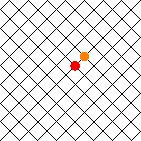
\includegraphics[scale=1.1]{figures/tikz/TFI/site_indices/site_index_b.pdf}
		}
	\end{minipage}
	\par\medskip
	\begin{minipage}{1.0\textwidth}
		\hspace{20pt}
		\begin{tikzpicture}[scale=1, trim axis left, trim axis right]
			\begin{axis}[xlabel=$t$, ylabel=$\langle\hat{\sigma}_z\rangle$, grid=both, grid style={gray!20}, every axis plot/.append style={very thick}, scale only axis, height=\globalQuenchLargeFieldFigureHeight, width=\globalQuenchLargeFieldFigureWidth, xmin=-0.05, xmax=1.05, ymin=0.9, ymax=1.05]
				%	
				\addplot[color = 5blue1]
				table[x=t_tenpy, y=sz_chi_16, col sep=space]{figures/plots/TFI/global_quench/data/global_quench_g_6.0_tenpy_site_index_5_5_0.txt};
				%\addlegendentry{$\chi= 16$}
				%	
				\addplot[color = 5blue2]
				table[x=t_tenpy, y=sz_chi_32, col sep=space]{figures/plots/TFI/global_quench/data/global_quench_g_6.0_tenpy_site_index_5_5_0.txt};
				%\addlegendentry{$\chi= 32$}
				%	
				\addplot[color = 5blue3]
				table[x=t_tenpy, y=sz_chi_64, col sep=space]{figures/plots/TFI/global_quench/data/global_quench_g_6.0_tenpy_site_index_5_5_0.txt};
				%\addlegendentry{$\chi= 64$}
				%	
				\addplot[color = 5blue4]
				table[x=t_tenpy, y=sz_chi_128, col sep=space]{figures/plots/TFI/global_quench/data/global_quench_g_6.0_tenpy_site_index_5_5_0.txt};
				%\addlegendentry{$\chi= 128$}
				%	
				\addplot[color = 5blue5]
				table[x=t_tenpy, y=sz_chi_256, col sep=space]{figures/plots/TFI/global_quench/data/global_quench_g_6.0_tenpy_site_index_5_5_0.txt};
				%\addlegendentry{$\chi= 256$}
				%
			\end{axis}%
			\begin{axis}[scale only axis, height=\globalQuenchLargeFieldFigureHeight, width=\globalQuenchLargeFieldFigureWidth, every axis plot/.append style={very thick}, xmin=-0.05, xmax=1.05, ymin=0.9, ymax=1.05]
				%	
				\addplot[color = 3red1]
				table[x=t_disoTPS, y=sz_disoTPS_D_2, col sep=space]{figures/plots/TFI/global_quench/data/global_quench_g_6.0_disoTPS_site_index_5_5_0.txt};
				%\addlegendentry{$D = 2$}
				%	
				\addplot[color = 3red2]
				table[x=t_disoTPS, y=sz_disoTPS_D_4, col sep=space]{figures/plots/TFI/global_quench/data/global_quench_g_6.0_disoTPS_site_index_5_5_0.txt};
				%\addlegendentry{$D = 4$}
				%	
				\addplot[color = 3red3]
				table[x=t_disoTPS, y=sz_disoTPS_D_6, col sep=space]{figures/plots/TFI/global_quench/data/global_quench_g_6.0_disoTPS_site_index_5_5_0.txt};
				%\addlegendentry{$D = 5$}
				%
			\end{axis}%
		\end{tikzpicture}%
		\quad
		\raisebox{34.2pt}
		{%
			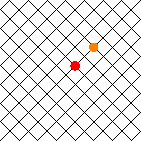
\includegraphics[scale=1.1]{figures/tikz/TFI/site_indices/site_index_c.pdf}
		}
	\end{minipage}
	\caption{In this figure we show the time evolution of the $\langle\hat{\sigma}_z\rangle$ expectation value of a spin in the middle of the lattice and its neighbouring spins. The position of the spins is visualized in the lattice next to the plots. As a model we use the TFI model in the paramagnetic phase with a transverse field of $g = 6$, put on an $8\times8$ diagonal square lattice containing in total $N = 128$ spins. We compute the time evolution once with DMRG on a MPS and once with disoTPS with the parameters given in the text.}
	\label{fig:disoTPS_time_evolution_g_6}
\end{figure}